\chapter{Two-source high harmonic generation}
\label{two_source}

\section{Introduction}
\label{intro_ts}

A common difficulty in working with extreme ultraviolet (XUV) light is the lack of efficient and broadband optics, especially beam splitters. In this chapter, I will introduce a method for generating two sources of XUV light by high harmonic generation using a \gls{swpg}.  This \gls{swpg} allows for the duplication of an \gls{ir} pulse, as well as precise and stable control of the relative phase between the duplicates of the input \gls{ir} pulse. The two most intense duplicates can generate harmonics which will interfere in the far-field. This can be thought of as an inline Mach-Zehnder interferometer with interferometric stability on sub-wavelength level of the high harmonic. The inherent stability of this two-source scheme will be utilized to measure both the real and imaginary parts of the refractive index of a medium.

\section{Theory}
\subsection{Laser beam shaping using diffractive optics}
\label{sec:beam_shaping}
%Describe general problem of beam shaping using DOEs. see \cite{romeroMathematicalAspectsLaser2010,romeroMathematicalTheoryLaser2010,romeroTheoryOptimalBeam2007}
%!!!!!!!!!!!!!!!!!!!!!!!!!!!!!!!!!!!!!!!!!!!!!!!!!!!!!!!!!!!!!!!!!!!!!!!!!!!!!!!!!!!!!!!!!!!!!!!!!!!!!!!!!!!!!!!!!!
%!!!!!!!!!!!!!!!!!!!!!!!!!!!!!!!!!COME BACK TO THIS SECTION LATER!!!!!!!!!!!!!!!!!!!!!!!!!!!!!!!!!!!!!!!!!!!!!!!!!!
%!!!!!!!!!!!!!!!!!!!!!!!!!!!!!!!!!!!!!!!!!!!!!!!!!!!!!!!!!!!!!!!!!!!!!!!!!!!!!!!!!!!!!!!!!!!!!!!!!!!!!!!!!!!!!!!!!!

In many experimental designs, it is advantageous to be able to shape the spatial intensity distribution of light to be something other than a typical Gaussian beam.  A common example of this is generating a beam with an approximately constant intensity across it's spatial profile (a flat-top beam).  For the experiments described herein, we will be interested in duplicating an input beam with relative phase control between the two duplicate beams.  Both of these examples are part of the general concept of laser beam shaping.  The challenge is to design an optical system such that given an input beam profile $I_{in}(x,y)$ we can generate the desired output beam profile $I_{out}(x,y)$. Ideally, this optical system is designed in such a way that it can be nearly lossless.\footnote{In the limit of geometric optics it is possible to make the optical system, in principle, lossless, however this is not generally possible when one considers the wave nature of light.}  The relevant optical system which will be used is shown in figure \ref{fig:beam_shaping_scheme}.  The system consists of a phase element which modifies the input field by $\phi(x,y)$ and a Fourier transform lens which adds a quadratic phase to the beam to focus it at the focal plane.  By appropriate choice of the phase profile of the phase element, one can produce the desired beam profile at the focal plane.


\begin{figure}
	\centering
	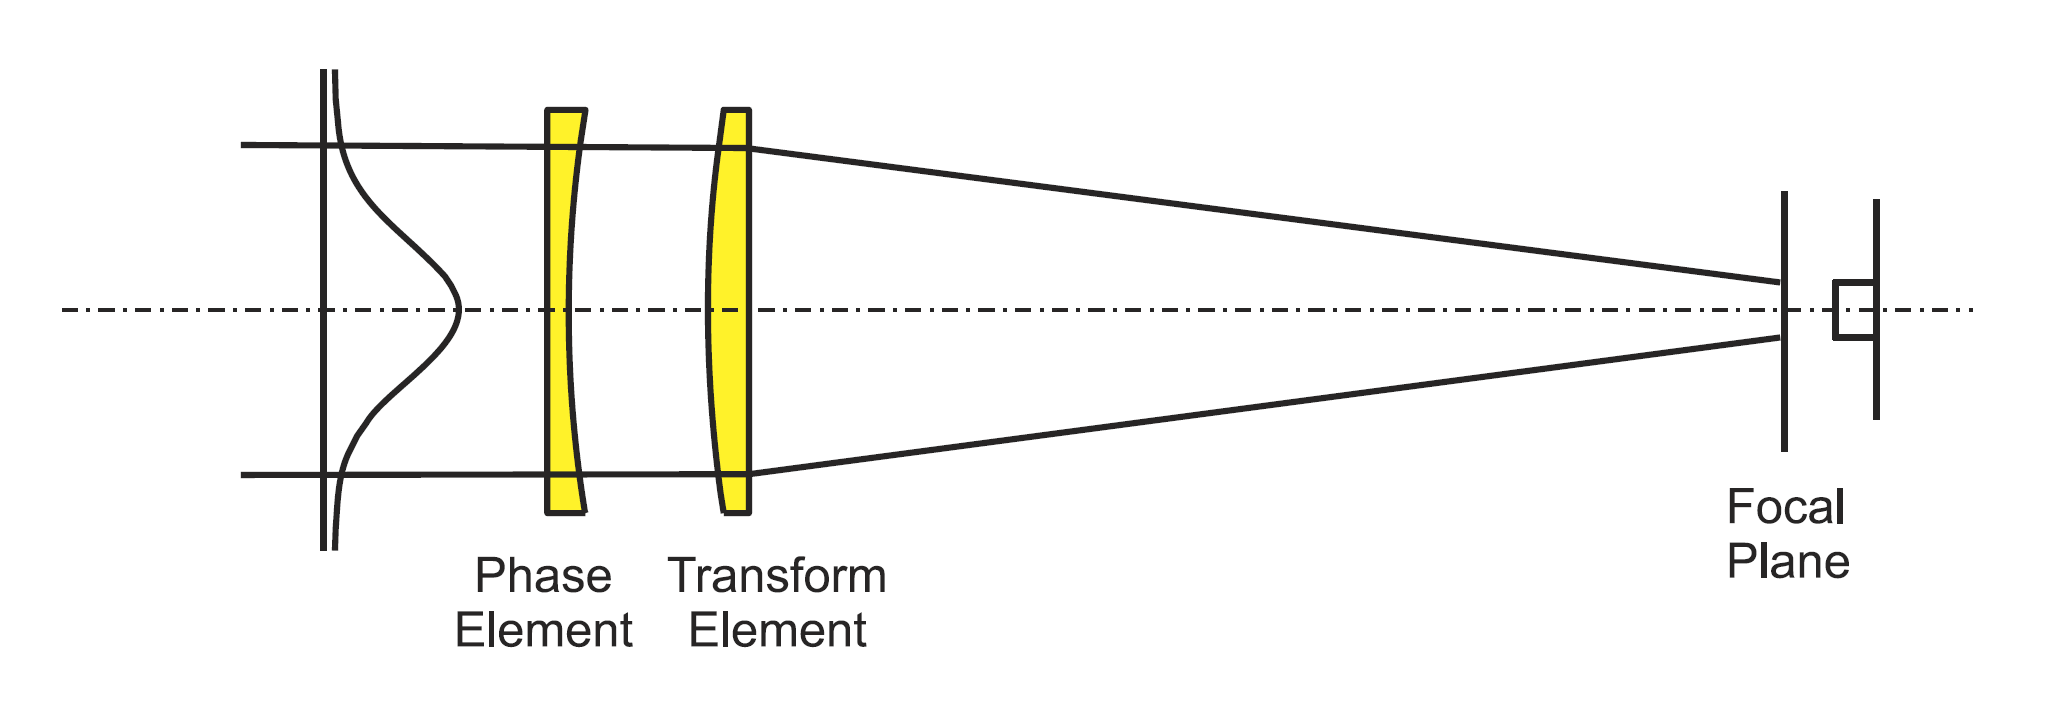
\includegraphics[width=0.9\textwidth]{figures/Two_source/romero_beam_shaping_schematic.png}
	\caption{Schematic demonstrating how to use a diffractive optical element to shape the beam profile at the focal plane. A collimated coherent beam is incident upon a diffractive optical element which shapes the phase of the incident beam, and then a lens is used as a transform element to Fourier transform the beam at the focal plane.  The intensity profile at the focal plane can be controlled by altering the spatial dependence of the phase imparted upon the incident beam by the phase element. Adapted from \cite{romeroMathematicalAspectsLaser2010}}
	\label{fig:beam_shaping_scheme}
\end{figure}


This problem can be theoretically described in terms of Fourier optics \cite{dickeyLaserBeamShaping2000, romeroMathematicalAspectsLaser2010, goodmanIntroductionFourierOptics2005}.  If one assumes that a field $u(x,y,0)$ is incident upon an an aperture at $z=0$, then the field for $z>0$ can be written under the Fresnel approximation by the Fresnel integral
\begin{equation}
\label{fresnel_integral}
	u(x,y,z)=\frac{i k}{2\pi z}e^{i k z}e^{i k (x^2+y^2)/2z}\int_{-\infty}^{\infty}\int_{-\infty}^{\infty}u(\xi,\eta,0) e^{ik(\xi^{2}+\eta^{2})/2z} e^{-ik(x\xi + y\eta)/z} \diff\xi\diff\eta
\end{equation}
where $u(\xi,\eta,0)$ is the incoming field and $k=2\pi/\lambda$ is the wavenumber.  Now, if one assumes that the phase element is placed at $z=0$, then immediately after passing through the thin phase element in Fig. \ref{fig:beam_shaping_scheme} the field is given by
\begin{equation}
	u(\xi,\eta,0)=f(\xi,\eta)e^{i\phi(\xi,\eta)}.
\end{equation} 
After propagating through the thin Fourier transform lens of focal length $f$, the field at the focal plane is now given by
\begin{equation}
\label{eqn:field_at_focus}
	u(x,y,f)=\frac{ik}{2\pi f}e^{ikf}e^{ik(x^2+y^2)/2f}\int_{-\infty}^{\infty}\int_{-\infty}^{\infty}f(\xi,\eta)e^{i\psi(\xi,\eta)}
	e^{-ik(x\xi + y\eta)/f}\diff\xi\diff\eta
\end{equation}
where
\begin{equation}
	\psi(\xi,\eta)=\phi(\xi,\eta) + k(\xi^2 + \eta^2)/2f.
\end{equation}

Now, the idea is to rewrite this field profile at the focal plane into a more intuitive form by introducing the equation
\begin{equation}
	g(\xi,\eta)=\frac{ik}{2\pi f}f(\xi,\eta)e^{i\psi(\xi,\eta)}.
\end{equation}
The Fourier transform of this function $g(\xi,\eta)$ is given by
\begin{equation}
\label{eqn:big_G}
	G(a,b)=\frac{ik}{2\pi f}\int_{-\infty}^{\infty}\int_{-\infty}^{\infty}f(\xi,\eta)e^{i\psi(\xi,\eta)}
	e^{-i(a\xi + b\eta)}\diff\xi\diff\eta.
\end{equation}
By setting $a=kx/f$ and $b=ky/f$ and taking the square complex modulus, one obtains the equation
\begin{equation}
	\rvert G(kx/f,ky/f)\rvert^{2} = \frac{k^2}{(2\pi f)^2} \bigg\rvert\int_{-\infty}^{\infty}\int_{-\infty}^{\infty}
	f(\xi,\eta)e^{i\psi(\xi,\eta)}e^{-ik(x\xi+y\eta)/f}\diff\xi\diff\eta\bigg\rvert^{2}.
\end{equation}
By comparing this equation with the square complex modulus of the field at the focal plane (equation \ref{eqn:field_at_focus}), one finds the relationship
\begin{equation}
\label{eqn:Fourier_focal_plane}
	\rvert u(x,y,f)\rvert^2 = \rvert G(kx/f,ky/f)\rvert^2.
\end{equation}

From this last equality we have shown that the intensity of the field at at the focal plane $\rvert u(z=f)\rvert^2$, is given by the Fourier transform of the combined phase imparted upon the incident field by both the phase element and the Fourier transform lens, $\rvert G\rvert^2$. So, if one wants a specific beam shape $Q(x,y)$ at the focal plane, then by tuning the frequency components of the phase imparted upon the beam $\phi(x,y)$ and the focal length $f$ used then one can achieve the desired beam profile, such that
\begin{equation}
\label{eqn:beam_shaping_equality}
	\rvert G(kx/f,ky/f)\rvert^2=Q(x,y).
\end{equation}
This problem is difficult in general, so the challenge in many beam shaping problems is to try and minimize the error between the true field and the desired field, and to further complicate the matter, many applications will require different notions of error to be used.  For example, if one needs the energy distribution to be as close as possible to the desired profile, then the $\ell_2$-norm would be appropriate.  However, if the maximum intensity is of concern, then the $\ell_\infty$-norm combined with the $\ell_2$-norm would be the appropriate notion of error.

It is possible to gain more insight into how difficult a beam shaping problem will be by reformulating the problem in terms of relevant length scales.  The idea is to introduce a dimensionless parameter whose magnitude will reflect the validity of underlying assumptions, and so for a given value of this parameter one can intuitively understand the performance (or lack thereof) of the beam shaping system.  This is done by reformulating the above situation in terms of the natural length scales of both the incoming field and the desired field at the focal plane
\begin{align}
	I_{\mathrm{input}} &= \rvert f(x,y)\rvert^2=\rvert\hat{f}(x/\sigma,y/\sigma)\rvert^2\\
	I_{\mathrm{desired}} &= Q(x,y)=\hat{Q}(x/d,y/d)
\end{align}
where $\sigma$ is the characteristic length scale of the input field (typically the beam radius) and $d$ is the characteristic length scale of the desired field.  By expressing the fields in this way, we can now introduce the dimensionless parameter
\begin{equation}
\label{eqn:beta_parameter}
	\beta=\frac{2\pi\sigma d}{\lambda f}.
\end{equation}
Using this dimensionless parameter, one can rewrite equations \ref{eqn:big_G} and \ref{eqn:beam_shaping_equality} as
\begin{align}
\label{eqn:new_G}
	G(\chi,\nu) &= \int_{-\infty}^{\infty}\int_{-\infty}^{\infty} g(\xi,\eta)e^{-i(\chi\xi+\nu\eta)}e^{i\beta\hat{\psi}(\xi,\eta)} \diff\xi\diff\eta\\
\label{eqn:beta_beam_shaping_equality}
	\rvert G(\chi, \nu)\rvert^2 &= \frac{4\pi^2 A}{\beta^2}Q(\chi/\beta,\nu/\beta)
\end{align}
where $\chi=x\sigma k /f$, $\nu=y\sigma k /f$, $A$ is a constant, and $\hat{\psi} = \beta\psi$. From equation \ref{eqn:new_G}, it is clear that the functions $g$ and $G$ are related by a Fourier transform, so they must obey the uncertainty relation given by
\begin{equation}
	\mu_g \mu_G\geq 1
\end{equation}
where $\mu$ is the second moment.  Now, if one were to choose the phase profile of the phase element $\phi(x,y)$ such that equation \ref{eqn:beta_beam_shaping_equality} is satisfied, then one finds that $\mu_G=\beta^2\mu_Q$.  This then leads to the inequality
\begin{equation}
\label{eqn:beta_inequalty}
	\beta^2 \mu_G\mu_Q\geq 1.
\end{equation}
It can be seen that for large vales of $\beta$ this inequality can be readily satisfied.  However, for very small values of $\beta$ this inequality cannot be met and it will not be possible to produce the desired beam profile.  From this, it can be seen that having a large value of $\beta$ makes the beam shaping problem more tractable.  The physical interpretation of $\beta$ is that is a measure of validity of geometric optics.  It can be shown that when $\beta$ is large a stationary phase method can be used to expand equation \label{eqn:new_G}, and the lowest order term can be derived using a geometric optics approximation and higher order terms are related to the effects of diffraction \cite{dickeyLaserBeamShaping2000, romeroMathematicalAspectsLaser2010}.

In this section, the general problem of laser beam shaping has been introduced and formulated as a problem in Fourier analysis, and by rewriting everything in terms of natural length scales we can infer which types of beam shaping problems will be more tractable using geometrical optics approximations.  The discussion so far has been kept very abstract, but in the next section the problem of interest will be introduced and these ideas will become more concrete.

\subsection{Beam splitting phase grating}
\label{sec:phase_grating}
Now that the general theory behind laser beam shaping has been introduced, we move on to the specific problem at hand.  The idea is to produce two nearly identical XUV beams through \gls{hhg} using two nearly identical \gls{ir} beams.  The challenge is how to produce two nearly identical \gls{ir} beams while minimizing the energy lost in the process.  An additional requirement is that we can control the relative phase between these two \gls{ir} beams.  All of these requirements can be met through the use of a beam splitting phase grating.

As shown in section \ref{sec:beam_shaping}, the beam shape at the focal plane of a lens can be controlled through appropriate choice of a phase element and the spatially dependent phase $\phi(x,y)$ which is imparted upon the incoming beam.  We will still consider the schematic shown in figure \ref{fig:beam_shaping_scheme}.  However, the phase element which will be considered in this section (the beam splitting phase grating) will only modify the phase in one dimension, $\phi(x,y)=\phi(x)$, and it will be a periodic function with a period of $d$, $\phi(x)=\phi(x+d)$. If we expand the function $P(x)=e^{i\phi(x)}$ in a Fourier expansion
\begin{align}
\label{eqn:Fourier_coeff_def}
	P(x) = \sum_{n=-\infty}^{\infty}a_n e^{\frac{i2\pi n x }{d}}\\
	a_n = \frac{1}{d}\int_{-d/2}^{d/2} P(\tilde{x})e^{\frac{-i2\pi n\tilde{x}}{d}}\diff\tilde{x},
\end{align}
then it can be shown (see Appendix \ref{app:SWPG}) that each of the Fourier coefficients represents a diffracted beam and the energy contained in each diffracted beam is given by the square complex modulus of the Fourier coefficient $\rvert a_n\rvert^2$.  Thus, by making our phase element in figure \ref{fig:beam_shaping_scheme} a phase grating, we have split the beam into many diffraction orders.  We have specified the period of the phase grating by requiring $\phi(x)=\phi(x+d)$, however we have not yet determined its shape.  This can be accomplished by specifying the distribution of energy into the various diffraction orders.  Since we want to split the incoming beam into two duplicate beams, we are searching for $d$-periodic function such that puts equal energy into two diffraction orders and a maximal amount of the input energy is put into those two orders. It can be shown (see Appendix \ref{app:SWPG}) that the $d$-periodic function which meets these criteria is a $0-\pi$ \gls{swpg} given by
\begin{equation}
\label{eqn:swpg}
	P(x,x_0) = \mathrm{sign}\Bigg( \cos\bigg( \frac{2\pi(x-x_0)}{d}\bigg)\Bigg)
\end{equation} 
where $x_0$ is an offset of position of the \gls{swpg} in the plane transverse to the optical axis. From this equation, it can be seen that the phase of the incoming beam is modulated by either $0$ or $\pi$, and this is shown in figure \ref{fig:swpg} for $x_0=0$ and $x_0=d/10$. 

\begin{figure}
	\centering
	\includegraphics[width=1.0\textwidth]{figures/Two_source/swpg.png}
	\caption{Plot of the phase function $\phi(x-x_0)$ in units of $\pi$ for a $0-\pi$ \gls{swpg} with a period of $d$.  The dark blue curve (light blue) shows the phase function for $x_0 = 0$ ($x_0=d/10$). }
	\label{fig:swpg}
\end{figure}

From equation \ref{eqn:Fourier_coeff_def}, we can calculate the Fourier coefficients $a_n(x_0)$ for the \gls{swpg} for $n=0$ and $n\neq0$.  These Fourier coefficients determines how the energy is distributed between the different diffraction orders.  For the zeroth-order case ($n=0$), we find that
\begin{equation}
\begin{aligned}
a_0(x_0) &= \frac{1}{d}\int_{-d/2}^{d/2} \mathrm{sign}\Bigg( \cos\bigg( \frac{2\pi(\tilde{x}-x_0)}{d}\bigg)\Bigg) \diff\tilde{x}\\
a_0(x_0) &=\frac{1}{d}\Bigg[ -\int_{-\frac{d}{2}}^{-\frac{d}{4}+x_0}\diff\tilde{x} 
+\int_{-\frac{d}{4}+x_0}^{\frac{d}{4}+x_0}\diff\tilde{x}
-\int_{\frac{d}{4}+x_0}^{\frac{d}{2}}\diff\tilde{x}
\Bigg]\\
a_0(x_0) &=0.
\end{aligned}
\end{equation}
This demonstrates that zero energy is put into the zeroth-order diffraction for the $0-\pi$ \swpg.  For the other diffraction orders, we find that
\begingroup
\allowdisplaybreaks
\begin{equation}
	\begin{aligned}
		a_n(x_0) &= \frac{1}{d}\int_{-d/2}^{d/2} \mathrm{sign}\Bigg( \cos\bigg( \frac{2\pi(\tilde{x}-x_0)}{d}\bigg)\Bigg) e^{\frac{-i2\pi n\tilde{x}}{d}}\diff\tilde{x}\\
		&=\frac{1}{d}\Bigg[ -\int_{-\frac{d}{2}}^{-\frac{d}{4}+x_0} e^{-\frac{i2\pi n x}{d}}\diff\tilde{x} 
		+\int_{-\frac{d}{4}+x_0}^{\frac{d}{4}+x_0} e^{-\frac{i2\pi n x}{d}}\diff\tilde{x}
		-\int_{\frac{d}{4}+x_0}^{\frac{d}{2}} e^{-\frac{i2\pi n x}{d}}\diff\tilde{x}
		\Bigg]\\
		&=\frac{1}{i2\pi n}\Bigg[
		e^{\frac{i\pi n}{2}-\frac{i2\pi n x_0}{d}} - e^{i n \pi}
		+ e^{\frac{i\pi n}{2}-\frac{i2\pi n x_0}{d}} - e^{-\frac{i\pi n}{2}-\frac{i2\pi n x_0}{d}}
		+e^{-i n \pi} - e^{-\frac{i\pi n}{2}-\frac{i2\pi n x_0}{d}}
		\Bigg]\\
		&=\frac{1}{i\pi n}\Bigg[e^{\frac{i\pi n}{2}-\frac{i2\pi n x_0}{d}}-e^{-\frac{i\pi n}{2}-\frac{i2\pi n x_0}{d}} \Bigg] = \frac{\sin (n\pi/2)}{n\pi/2}e^{-i\frac{2\pi n x_0}{d}}\\
		a_n(x_0) &= \mathrm{sinc}(\frac{n\pi}{2})e^{-i n \frac{2\pi x_0}{d}}.
	\end{aligned}
\end{equation}
\endgroup
Since $\mathrm{sinc}(n\pi/2)=0$ for even $n$, we see that only the odd orders of diffraction from the \gls{swpg}  are populated. The distribution of energy between the different diffraction orders is plotted in figure \ref{fig:a_n}, and from this figure it is immediately clear that our choice of the $0-\pi$ \gls{swpg} has succeeded in putting most of the input energy equally into two diffraction orders, namely the $\pm1$ orders.  The efficiency of this phase grating can be defined as
\begin{equation}
	\eta=\rvert a_1\rvert^2 + \rvert a_{-1}\rvert^2 =\frac{8}{\pi^2}\approx 0.8106,
\end{equation} 
which means that approximately $81\%$ of the input energy will be put into the two orders that we want.  It should be noted that $\sum_{n}\rvert a_n\rvert^2=1$, which means that while we can't get perfect conversion of energy into two orders this is still a lossless design.
\begin{figure}
	\centering
	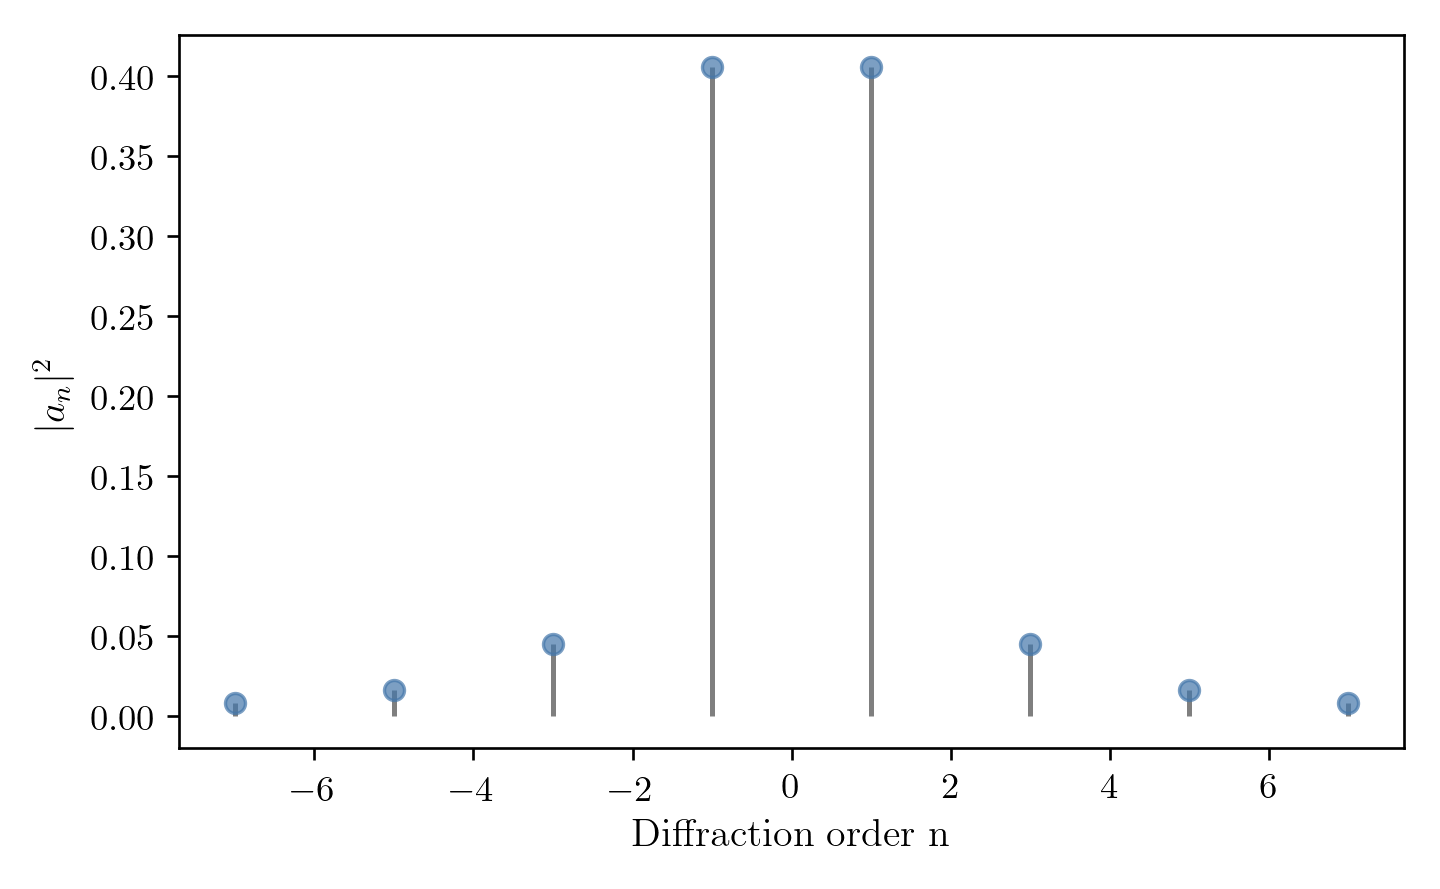
\includegraphics[width=1.0\textwidth]{figures/Two_source/a_n.png}
	\caption{Square complex modulus of the Fourier coefficients $a_n$ of the $0-\pi$ \gls{swpg}. The square complex modulus is proportional to the energy put into each diffraction order.  As can be seen from figure, the $\pm1$ orders have the most energy put into them at $4/\pi^2\approx41.1\%$ each.  All even orders have zero energy.}
	\label{fig:a_n}
\end{figure}

A very important feature of the \gls{swpg}


\begin{figure}
	\centering
	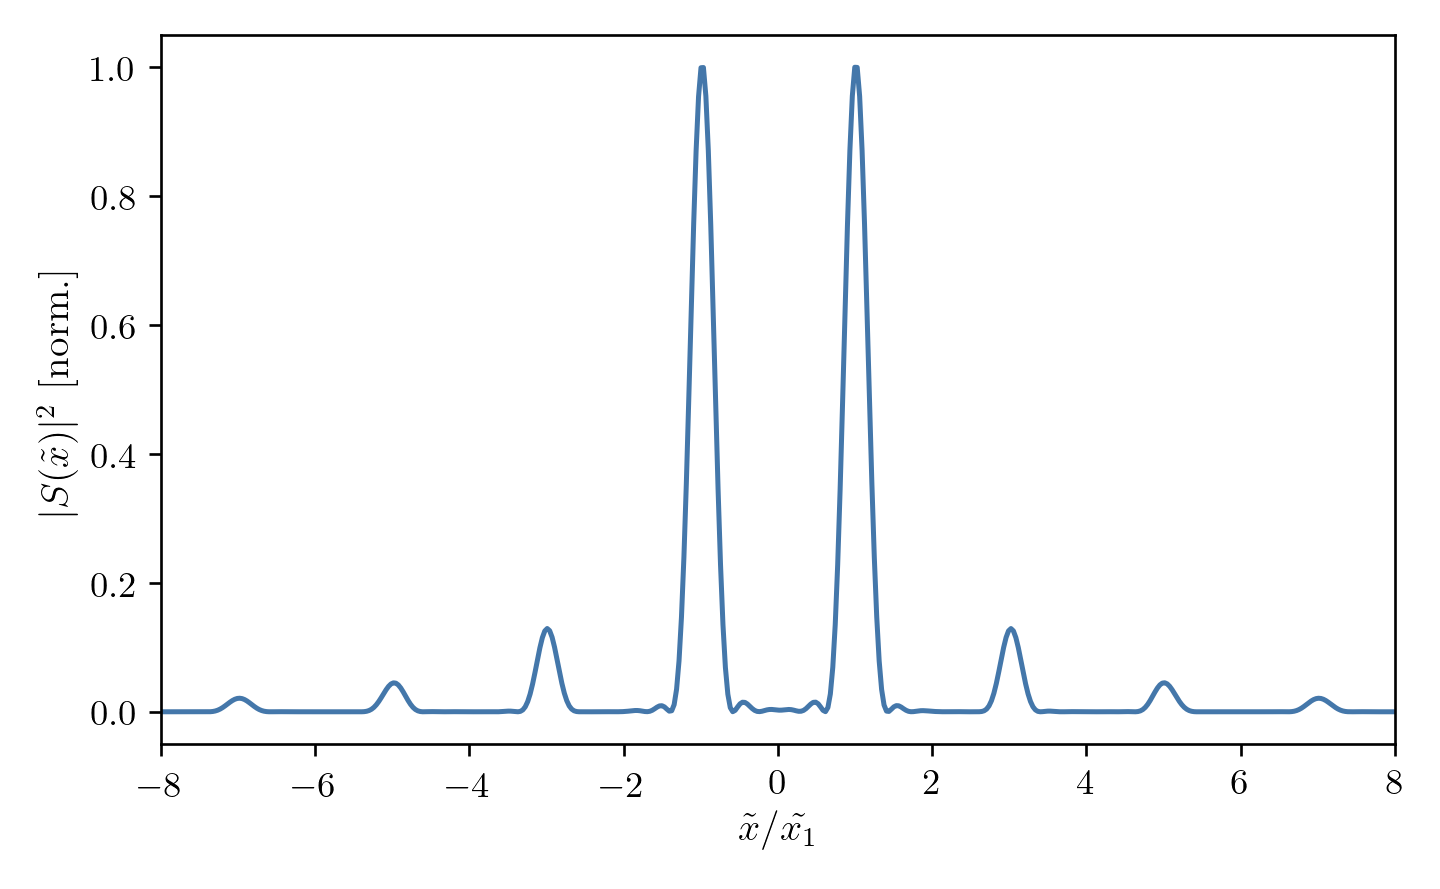
\includegraphics[width=1.0\textwidth]{figures/Two_source/focus_intensity.png}
	\caption{Intensity profile $S(\tilde{x})$ at the focal plane. Horizontal units are scaled by the spacing between orders, $\tilde{x_1}=\lambda f/d$.  Calculated by numerically propagation using Fresnel integral.}
	\label{fig:s^2}
\end{figure}

\begin{figure}
	\centering
	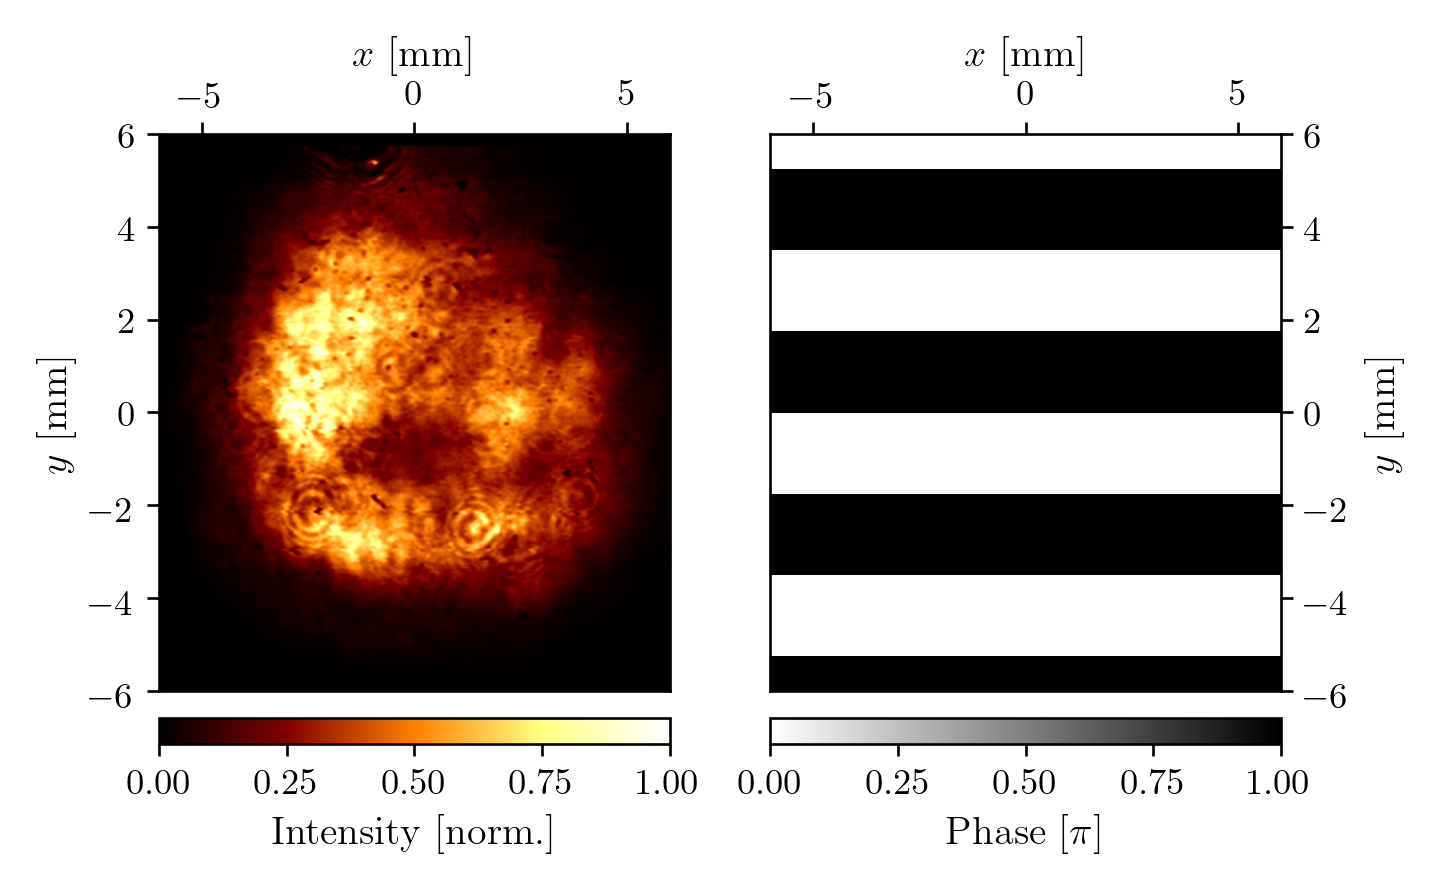
\includegraphics[width=1.0\textwidth]{figures/Two_source/LP_images.png}
	\caption{Intensity profile of the input beam measured by a thermal camera. Phase imparted by \gls{swpg}}
	\label{fig:LP_inputs}
\end{figure}

\subsection{Imperfect phase grating}
\section{Two-source high harmonic generation}


\begin{equation}
\label{eq:field}
S(x) = \sum_{n} E(x - x_{n})
\end{equation}






\begin{figure}
	\centering
	\begin{subfigure}[b]{0.45\textwidth}
		\caption{}
		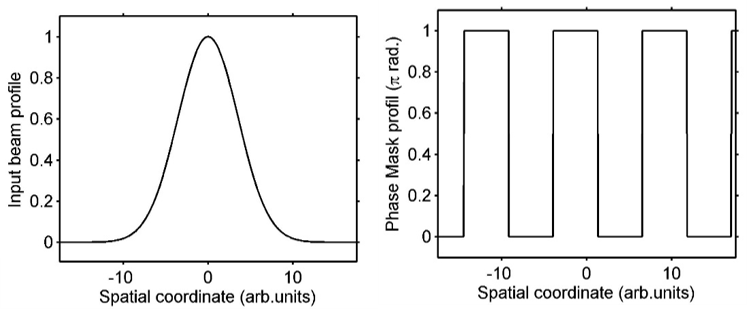
\includegraphics[width=\textwidth]{figures/Two_source/spatial_profile}
		\label{fig:spatial_profile}
	\end{subfigure}
	\begin{subfigure}[b]{0.45\textwidth}
		\caption{}
		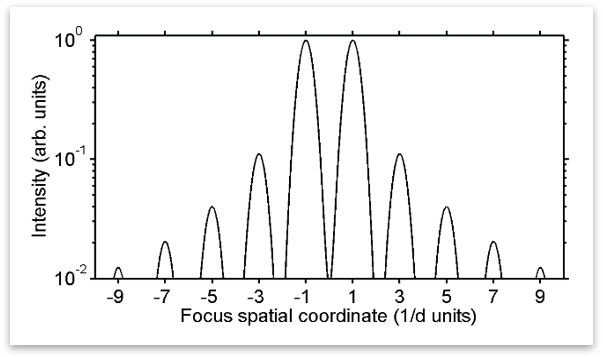
\includegraphics[width=\textwidth]{figures/Two_source/focus_profile}
		\label{fig:focus_profile}
	\end{subfigure}
	\caption{(a) Two-channel model for Feshbach resonance.  Incident atoms in the entrance channel (the open channel) couple to a bound state of energy $E_{c}$ supported by the closed channel.  Since collisions take place for $E\rightarrow 0$, tuning $E_{c}$ to 0 allows for the resonant coupling to occur. (b) Scattering length near a resonance where a bound state crosses the scattering threshold. Inset shows the quadratic behavior of the binding energy near the resonance.}
\end{figure}


\begin{equation}
	\begin{aligned}
    	I_{IR} &= a + b\times\cos\left(\phi(x_{0})\right)\\
     	I_{q} &= \alpha_q\times a^{q} \left(1+N_{q}\frac{b}{a}\cos\left(\phi(x_{0})\right)\right) + o(b\times a^{q-1})\\
	\end{aligned}
\end{equation}
\begin{equation}
	\begin{aligned}
		I_{IR}(\tilde{x}_{1},x_{0}) &= \left|\tilde{S}(\tilde{x}_{1},x_{0})\right|^{2} \\
		&= \left|a_{-1}\tilde{E}(2\tilde{x}_{1})+a_{0}\tilde{E}(\tilde{x}_{1})+a_{1}\tilde{E}(0)+a_{3}\tilde{E}(2\tilde{x}_{1})\right|^{2}\\
     &= \left|a_{0}\tilde{E}(\tilde{x}_{1})+a_{1}\tilde{E}(0)\right|^{2}\\
	\end{aligned}
\end{equation}
\begin{equation}
	\begin{aligned}
		 I_{IR}(\tilde{x}_{1},x_{0}) &=\left|\tilde{E}(0)\right|^{2}\left|\frac{2}{\pi}\sin\left(\xi\frac{\pi}{2}\right)e^{i(\xi\frac{\pi}{2}-\phi_{1})}+\cos\left(\xi\frac{\pi}{2}\right)e^{i\xi\frac{\pi}{2}}\frac{\tilde{E}(\tilde{x}_{1})}{\tilde{E}(0)} -  \frac{2\sin\left(\xi\frac{\pi}{2}\right)}{\pi}e^{i(\xi\frac{\pi}{2}+\phi_{1})}\frac{\tilde{E}(2\tilde{x}_{1})}{\tilde{E}(0)} + \frac{2\sin\left(\xi\frac{\pi}{2}\right)}{3\pi}e^{i(\xi\frac{\pi}{2}-3\phi_{1})}\frac{\tilde{E}(2\tilde{x}_{1})}{\tilde{E}(0)}\right|^{2}\\
	\end{aligned}
\end{equation}
\begin{equation}
	\begin{aligned}
		I_{IR}(\tilde{x}_{1},x_{0})  &= \left|\tilde{E}(0)\frac{2}{\pi}\sin\left(\xi\frac{\pi}{2}\right)\right|^{2}\left|e^{-i\phi_{1}}+\frac{\pi}{2\tan\left(\xi\frac{\pi}{2}\right)}\frac{\tilde{E}(\tilde{x}_{1})}{\tilde{E}(0)} -e^{i\phi_{1}}\frac{\tilde{E}(2\tilde{x}_{1})}{\tilde{E}(0)} +  \frac{e^{-3i\phi_{1}}}{3}\frac{\tilde{E}(2\tilde{x}_{1})}{\tilde{E}(0)}\right|^{2}\\
		&= \left|\tilde{E}(0)\frac{2}{\pi}\sin\left(\xi\frac{\pi}{2}\right)\right|^{2}\left(1+\frac{\pi}{\tan\left(\xi\frac{\pi}{2}\right)}\frac{\tilde{E}(\tilde{x}_{1})}{\tilde{E}(0)}\cos(\phi_{1})-\frac{4}{3}\frac{\tilde{E}(2\tilde{x}_{1})}{\tilde{E}(0)}\cos(2\phi_{1})\right)\\
		I_{IR}(\tilde{x}_{-1},x_{0}) &= \left|\tilde{S}(\tilde{x}_{-1},x_{0})\right|^{2} \\
		 &= \left|a_{-1}\tilde{E}(0)+a_{0}\tilde{E}(\tilde{x}_{1})\right|^{2}\\
		&= \left|\tilde{E}(0)\right|^{2}\left|-\frac{2}{\pi}\sin\left(\xi\frac{\pi}{2}\right)e^{i(\xi\frac{\pi}{2}+\phi_{1})}+\cos\left(\xi\frac{\pi}{2}\right)e^{i\xi\frac{\pi}{2}}\frac{\tilde{E}(\tilde{x}_{1})}{\tilde{E}(0)}+\frac{2\sin\left(\xi\frac{\pi}{2}\right)}{\pi}e^{(\xi\frac{\pi}{2}-\phi_{1})}\frac{\tilde{E}(2\tilde{x}_{1})}{\tilde{E}(0)} -  \frac{2\sin\left(\xi\frac{\pi}{2}\right)}{3\pi}e^{(\xi\frac{\pi}{2}+3\phi_{1})}\frac{\tilde{E}(2\tilde{x}_{1})}{\tilde{E}(0)}\right|^{2}\\
      &= \left|\tilde{E}(0)\frac{2}{\pi}\sin\left(\xi\frac{\pi}{2}\right)\right|^{2}\left|e^{-i\phi_{1}}-\frac{\pi}{2\tan\left(\xi\frac{\pi}{2}\right)}\frac{\tilde{E}(\tilde{x}_{1})}{\tilde{E}(0)} -e^{i\phi_{1}}\frac{\tilde{E}(2\tilde{x}_{1})}{\tilde{E}(0)} +  \frac{e^{-3i\phi_{1}}}{3}\frac{\tilde{E}(2\tilde{x}_{1})}{\tilde{E}(0)}\right|^{2}\\
      &= \left|\tilde{E}(0)\frac{2}{\pi}\sin\left(\xi\frac{\pi}{2}\right)\right|^{2}\left(1-\frac{\pi}{\tan\left(\xi\frac{\pi}{2}\right)}\frac{\tilde{E}(\tilde{x}_{1})}{\tilde{E}(0)}\cos(\phi_{1})-\frac{4}{3}\frac{\tilde{E}(2\tilde{x}_{1})}{\tilde{E}(0)}\cos(2\phi_{1})\right)\\
      %\forall n \in \mathbb{Z}, a^{\xi}_{2n+1}(x_{0}) &= \frac{2\sin\left(\xi\frac{\pi}{2}\right)}{(2n+1)\pi}e^{i(\xi\frac{\pi}{2}-(2n+1)\phi_{1})} \\
     a^{\xi}_{0}(x_{0}) &= \cos\left(\xi\frac{\pi}{2}\right)e^{i\xi\frac{\pi}{2}}
     \end{aligned}
\end{equation}


\begin{figure}
	\centering
	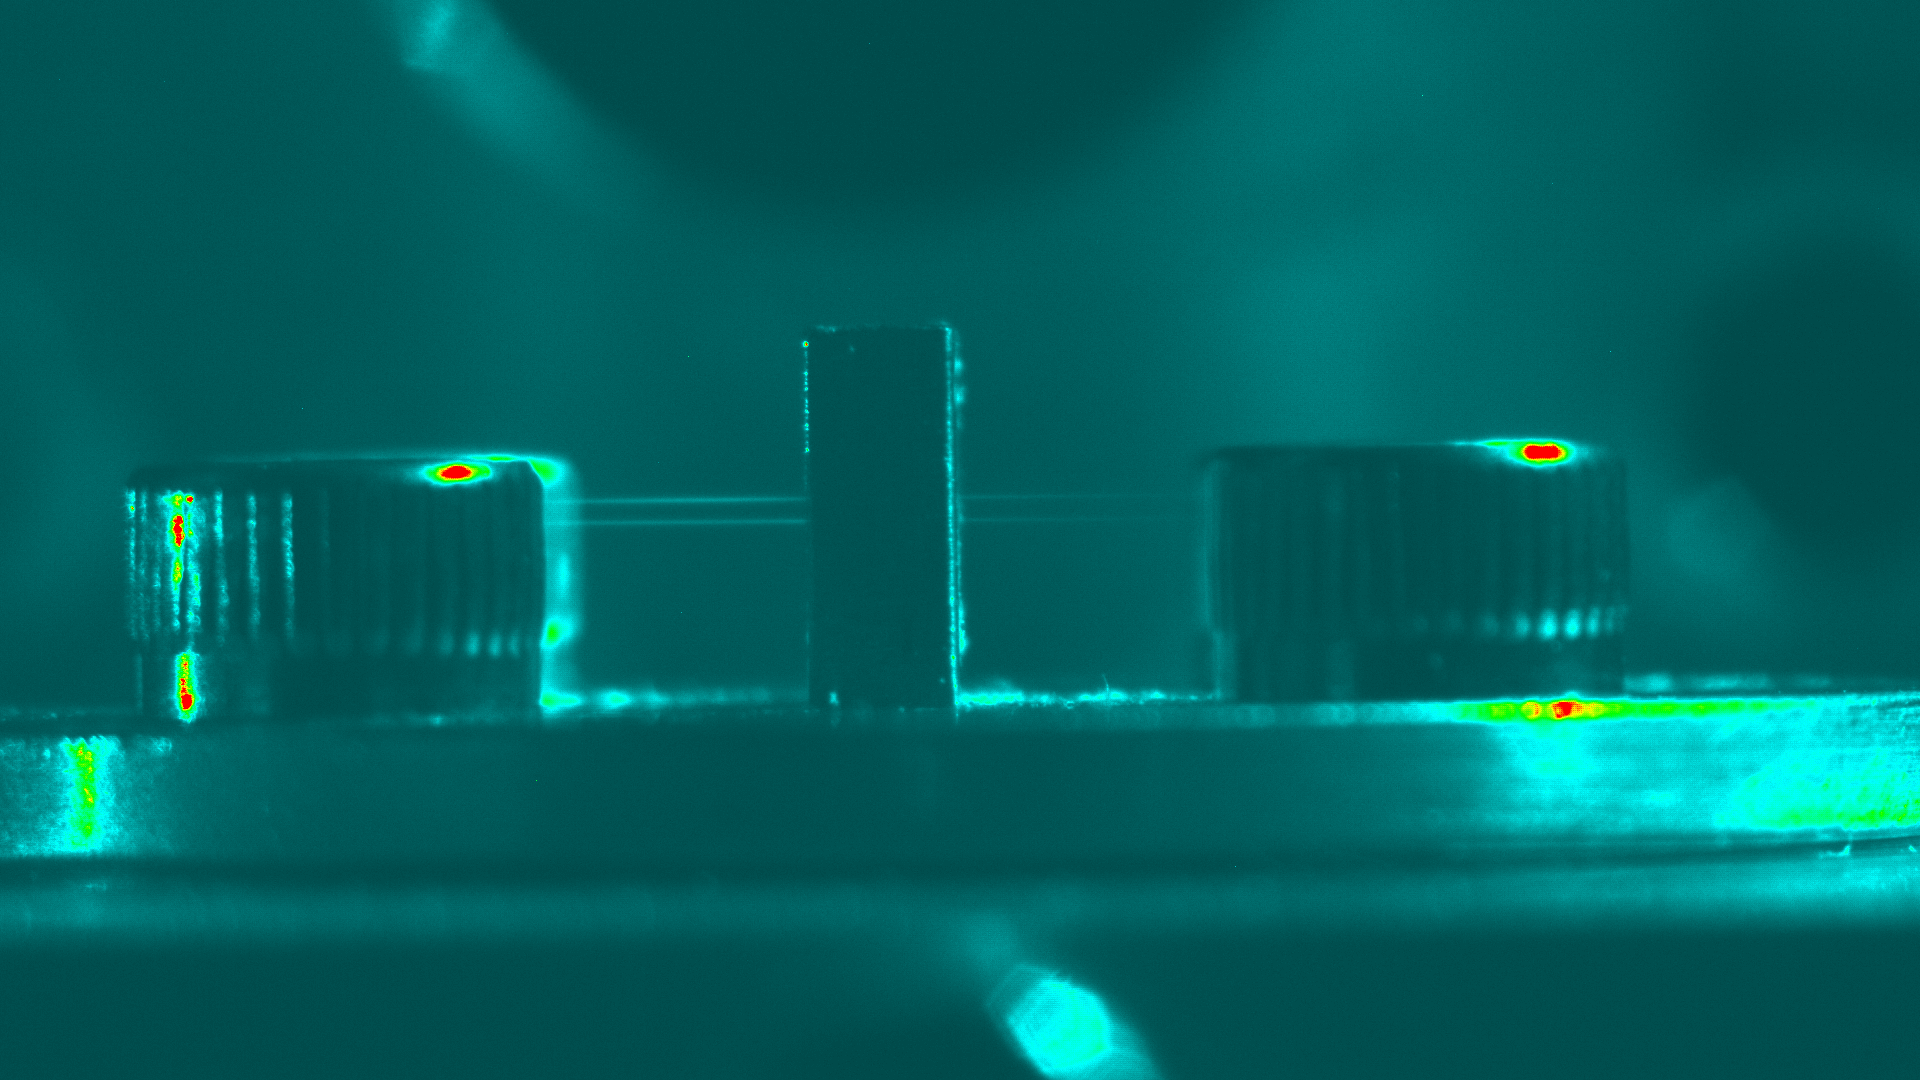
\includegraphics[width=0.9\textwidth]{figures/Two_source/ts_filament_gas_cell.png}
	\caption{Camera image of two sources generating a filament in a gas cell. Image was taken while chamber was vented and at ambient pressure.}
	\label{ts_filament}
\end{figure}

%\lipsum

\begin{figure}
	\centering
	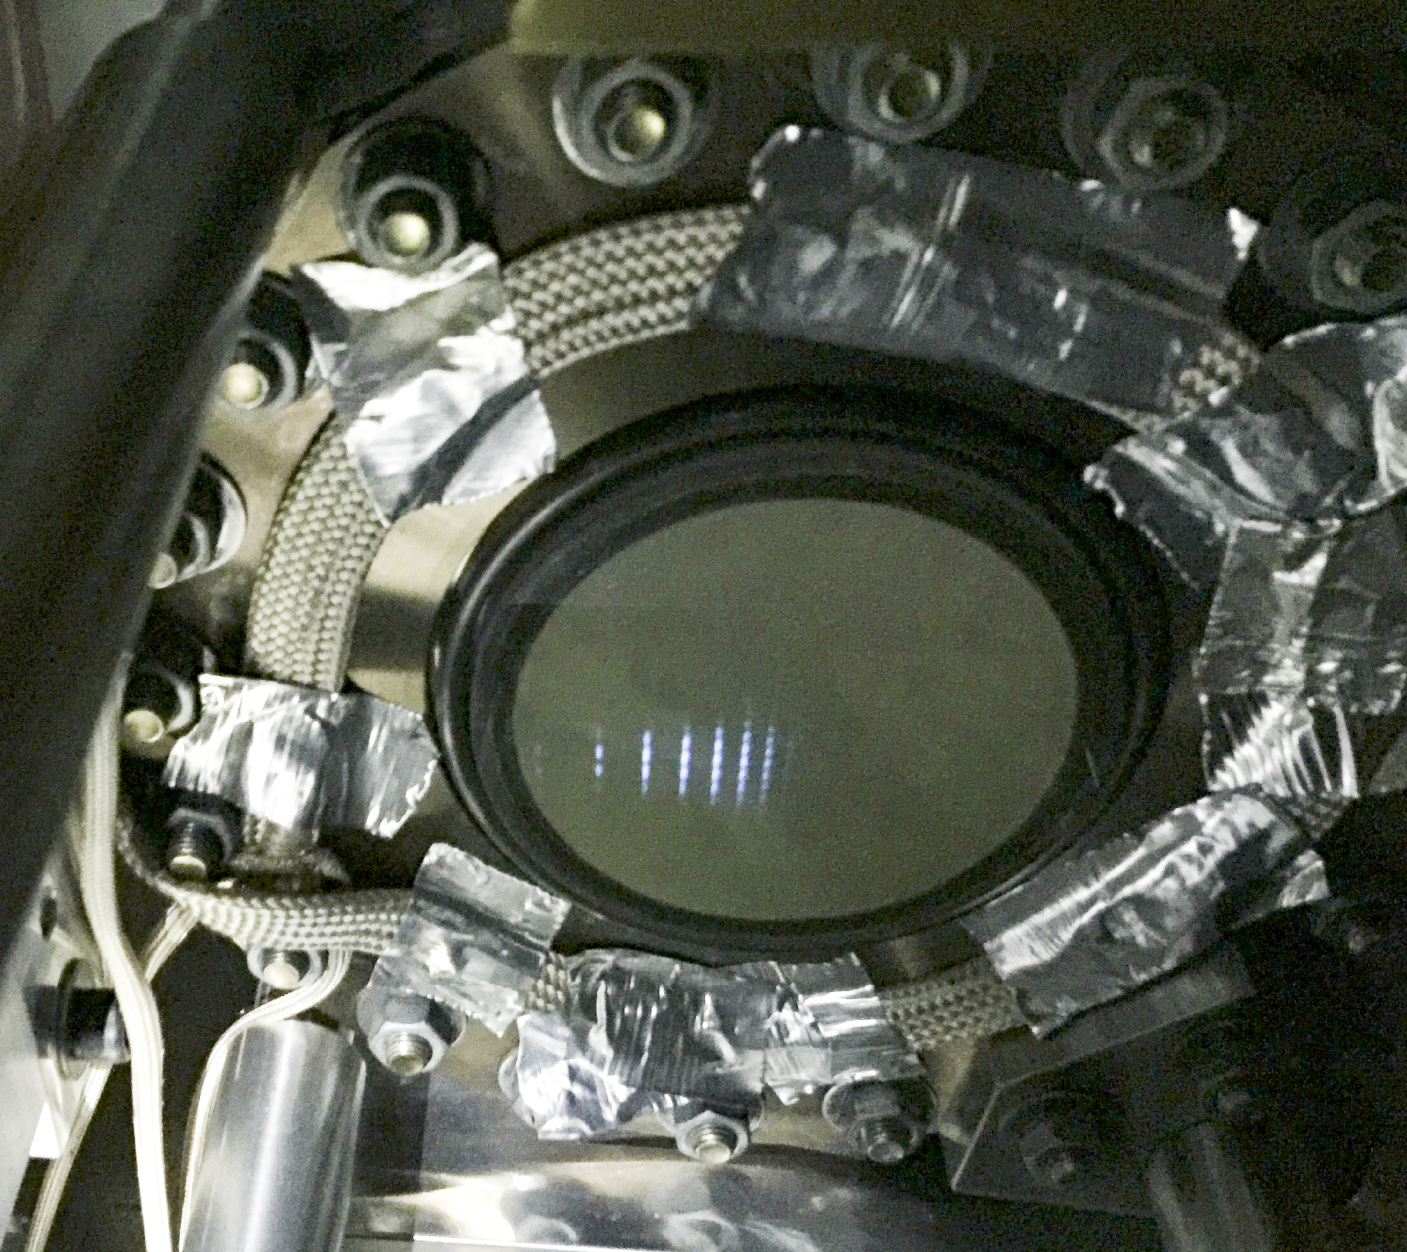
\includegraphics[width=0.9\textwidth]{figures/Two_source/MCP_ts_harmonics.png}
	\caption{Camera image of the output of the phosphor screen.  Harmonics are visible by eye.}
	\label{MCP_ts_harmonics}
\end{figure}


%\lipsum